\section{Adria Track}
%
In this section, the author describes the approach and report the results for the most challenging example, a real race track. Specifically, the circuit considered is the Adria International Raceway (figure \ref{fig:AdriaTrackpng}) located in north of Italy in Rovigo province. This is the same circuit used by Bobbo Simon \textit{et al.}\cite{simon2008application} in their publication. Therefore some confronts can be made.\\
The circuit in compose mainly of $8$ turns as indicated in figure \ref{fig:AdriaTrackpng}. However, the circuit has been described as a sum of section of constant curvature with fixed width ($12\;\si{\metre}$).
%
\begin{figure}[ht!]
    \centering
    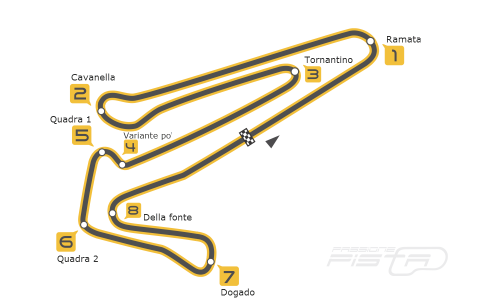
\includegraphics[width=0.7\linewidth]{Circuit/adria_vettoriale.png}
    \caption{Track of Adria courtesy of \href{http://www.passionepista.it/circuiti/descrizione/7-autodromo_di_adria}{passionepista.it}}
    \label{fig:AdriaTrackpng}
\end{figure}
%
\subsection{Solution approach}
%
This particular example inspired the author to develop the custom technique for optimal control problem initialisation described in chapter \ref{Ch:OCIni}. In fact, the author encounter many difficulties solving the OCP since it was not converging. The problem is particularly difficult because of its high non linearity and a large number of differential equations and constraints making the problem unstable.\\
The solutions strategy adopted is the same as in the U-shape turn and the S-shape turn. \\
The step 0 is to find a suitable solution that deviate as little as possible from the steady state. In particular, the important part is the minimisation of almost all velocities and accelerations. For instance, the square of rolling velocity and acceleration, steering velocity and suspensions velocities are minimised. This Produce a smooth motion that can be associated with a quasi-steady state. In fact there is a variation in longitudinal and lateral velocity as well as in the yaw rate.
As previously mentioned not all steady state condition are tracked. Specifically, $u$, $v$ and $\Omega$ are left free. This, along with a small weight to the minimum time, allow to reach a first solution.\\
The step 1 is pushing the steady state condition to zero while increasing the weight of the minimum time up to $1$.\\
The the $2^{nd}$ problem is to approach the initial and final condition, while keeping the starting one fixed.\\
At step 3 the initial conditions are slowly liberated from the constraints in the mayer term.\\
Last step is pushing the boundary and the tolerances on penalties and control limits.
%
\subsection{Results and comparison}
%
The main result of the single models are reported in appendix \ref{app:Adria} for space reasons.\\
Here the models behaviour are compared in their performances. As expected the velocity profiles of all four models are fairly close to each other (figure \ref{fig:AdriaUconfront}).\\
%
\begin{figure}[!htb]
    \centering
    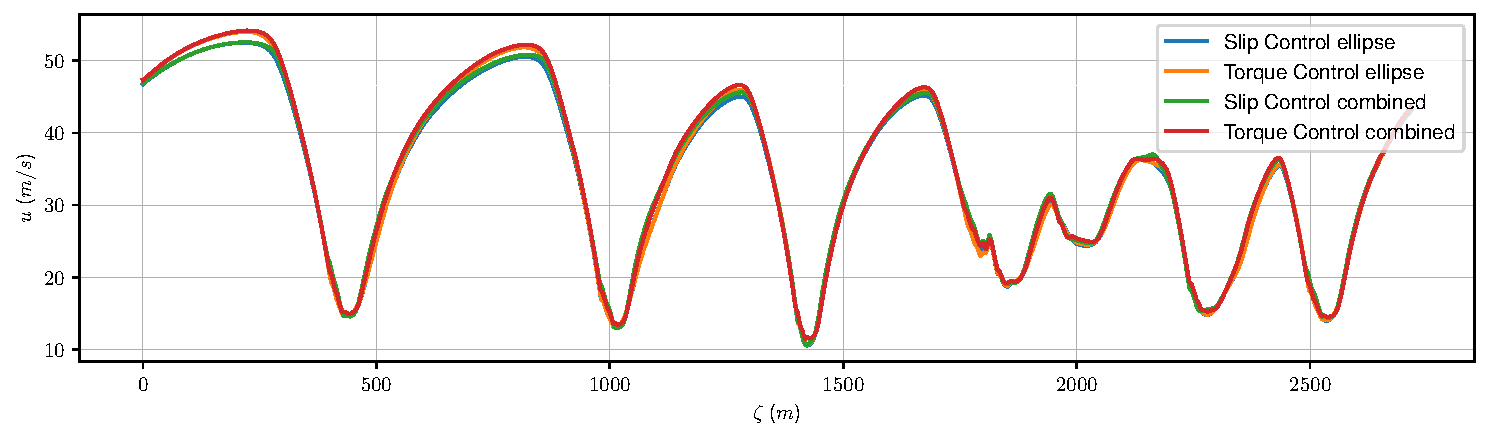
\includegraphics[width=\linewidth]{Circuit/u_P_confront.pdf}
    \caption{Longitudinal velocity confront}
    \label{fig:AdriaUconfront}
\end{figure}\\
%
The same can be said fot the rolling angle $phi$ and the deviation from the centreline respectively in figure \ref{fig:AdriaPHIconfront} and \ref{fig:AdriaNconfront}. It is important to highlight that in the straight sections the similarity between all models is strong, while the differences raises at the entering and at the exit of the turns. This ,of course, depend on how aggressive is the manoeuvre.\\
%
\begin{figure}[!htb]
    \centering
    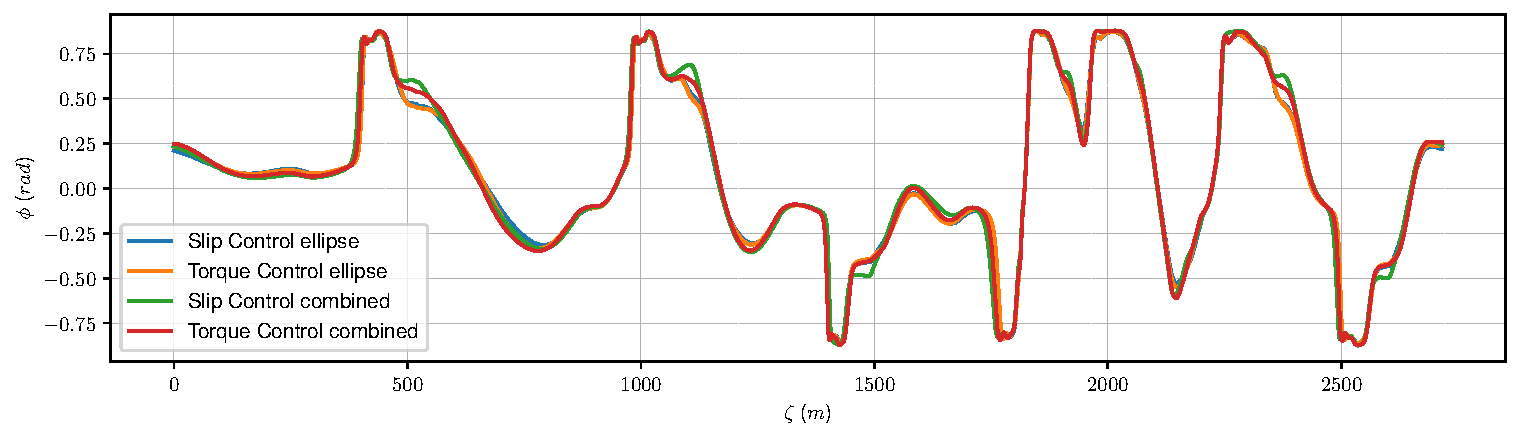
\includegraphics[width=\linewidth]{Circuit/phi_P_confront.pdf}
    \caption{Roll angle confront}
    \label{fig:AdriaPHIconfront}
\end{figure}
%
%
\begin{figure}[!htb]
    \centering
    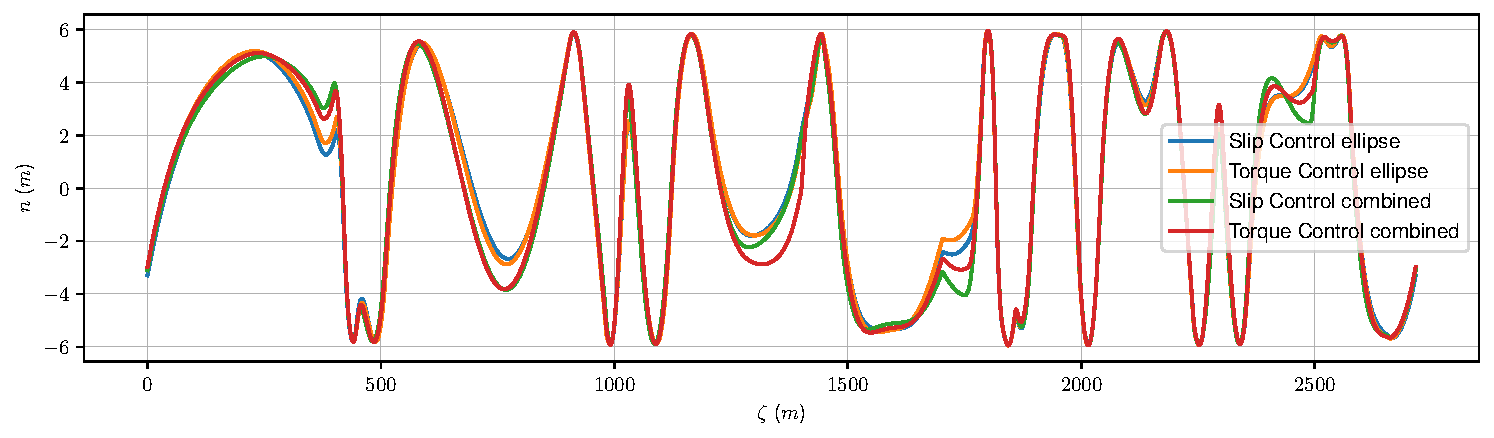
\includegraphics[width=\linewidth]{Circuit/n_P_confront.pdf}
    \caption{Centreline deviation confront}
    \label{fig:AdriaNconfront}
\end{figure}\\
%
Another key aspect of the simulation is the strong similarity between the ellipse of adherence in the four cases. as represented in figure \ref{fig:AdriaEF} for the front wheel and figure \ref{fig:AdriaER} for the rear wheel.\\
%
\begin{figure}[!htb]
    \centering
    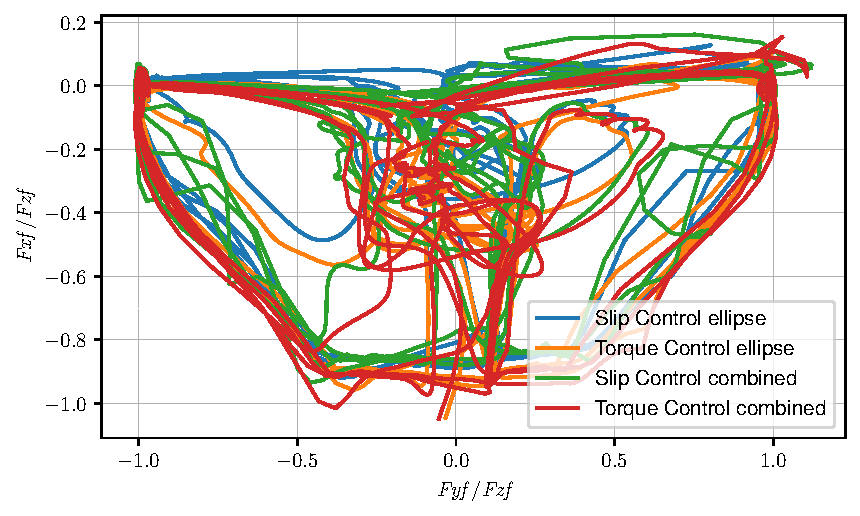
\includegraphics[width=0.6\linewidth]{Circuit/EFront_P_confront.pdf}
    \caption{Ellipse of adherence front wheel confront}
    \label{fig:AdriaEF}
\end{figure}
%
\begin{figure}[!htb]
    \centering
    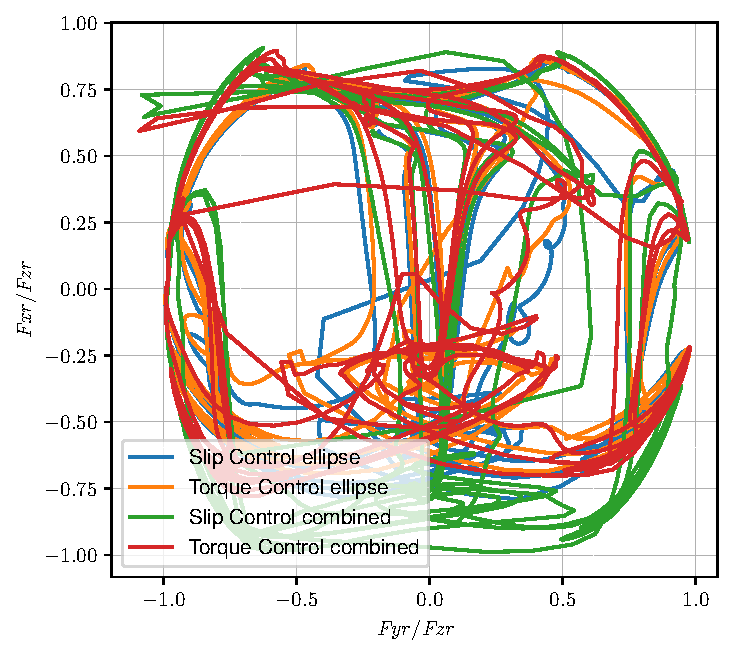
\includegraphics[width=0.6\linewidth]{Circuit/ERear_P_confront.pdf}
    \caption{Ellipse of adherence rear wheel confront}
    \label{fig:AdriaER}
\end{figure}\\
%
As it can be seen from the two ellipse the maximum performance in acceleration is almost the same. It follows almost perfectly the border of maximum performances and it is truncated in the upper part for two main reasons. The first is the limit imposed on the vertical to prevent wheelie condition and the second is the aerodynamic drag. A remarkable result is that the combined tyre model and the constrained ellipse of adherence produce the same performance.\\
There are some points that exit the border of the ellipse. Those are there only in the torque control model and can be motivated with the fact dynamic of the slip imposed by the torque control. The OCP in those point reach a bound with high penalty which reflects in a fast and aggressive response.\\
In braking condition it can be observed that the slip control use the rear wheel much more. This is in fact a reflection of the vertical load at the rear wheel in braking.\\
% As it is shown in figure \ref{fig:AdriaAR} the rear tyre reach the peak longitudinal performance.\\
% %
% \begin{figure}[!htb]
%     \centering
%     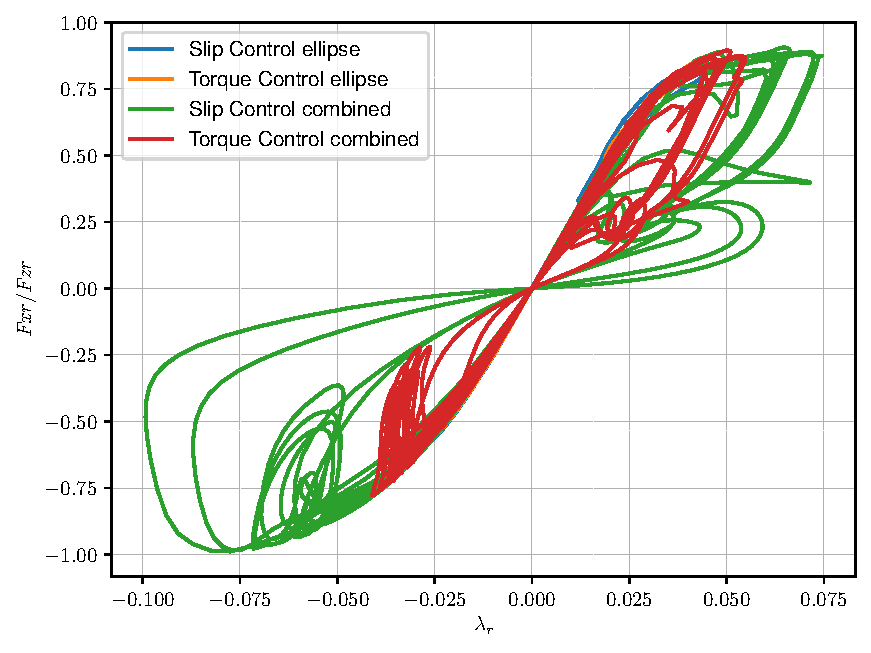
\includegraphics[width=0.5\linewidth]{Circuit/RearAdherence_P_confront.pdf}
%     \caption{Longitudinal tyre force vs slip rear wheel confront}
%     \label{fig:AdriaAR}
% \end{figure}\\
%
In figure \ref{fig:AdriaEF} the similarity is much stronger. All model reach almost the same performance that do not have the shape of an ellipse. This could seem a strange results, but it is motivated. In fact, in the constraints of the OCP there is a bound to impose a minimum in both front and rear vertical load. In this case, the constraint avoid the stoppie condition (wheelie of the rear wheel) and therefore the maximum performance in braking is limited. This is reflected in the ellipse of adherence with a truncation of the lower part.\\
Another important aspect to highlight is the respect of the bound on the maximum torque deriving from the ICE power. In figure \ref{fig:AdriaTorqueConfront} are reported the torque applied confronted with the torque curve of the engine for each gear.\\
%
\begin{figure}[!htb]
    \centering
    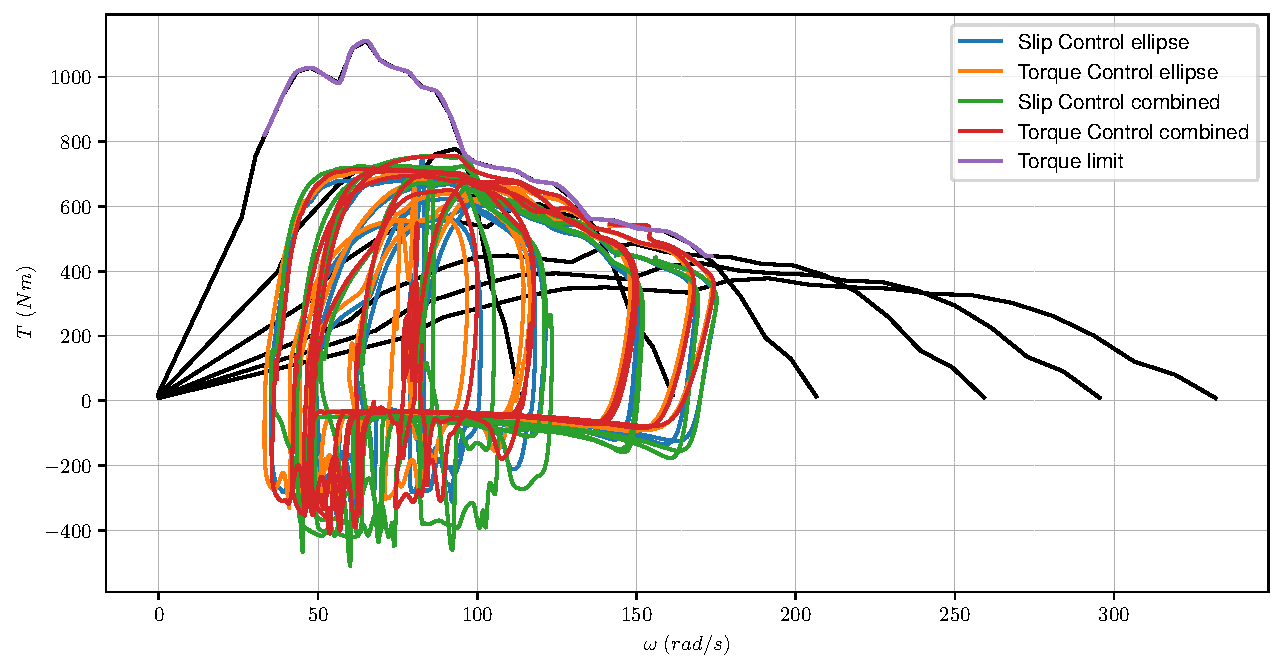
\includegraphics[width=0.8\linewidth]{Circuit/Torque_P_confront.pdf}
    \caption{Trajectory}
    \label{fig:AdriaTorqueConfront}
\end{figure}\\
%
%
As previously addressed the trajectory in most part is indistinguishable. For completeness the comparison of the trajectories is reported in figure \ref{fig:AdriaTrajConfront}
%
\begin{figure}[!h]
    \centering
    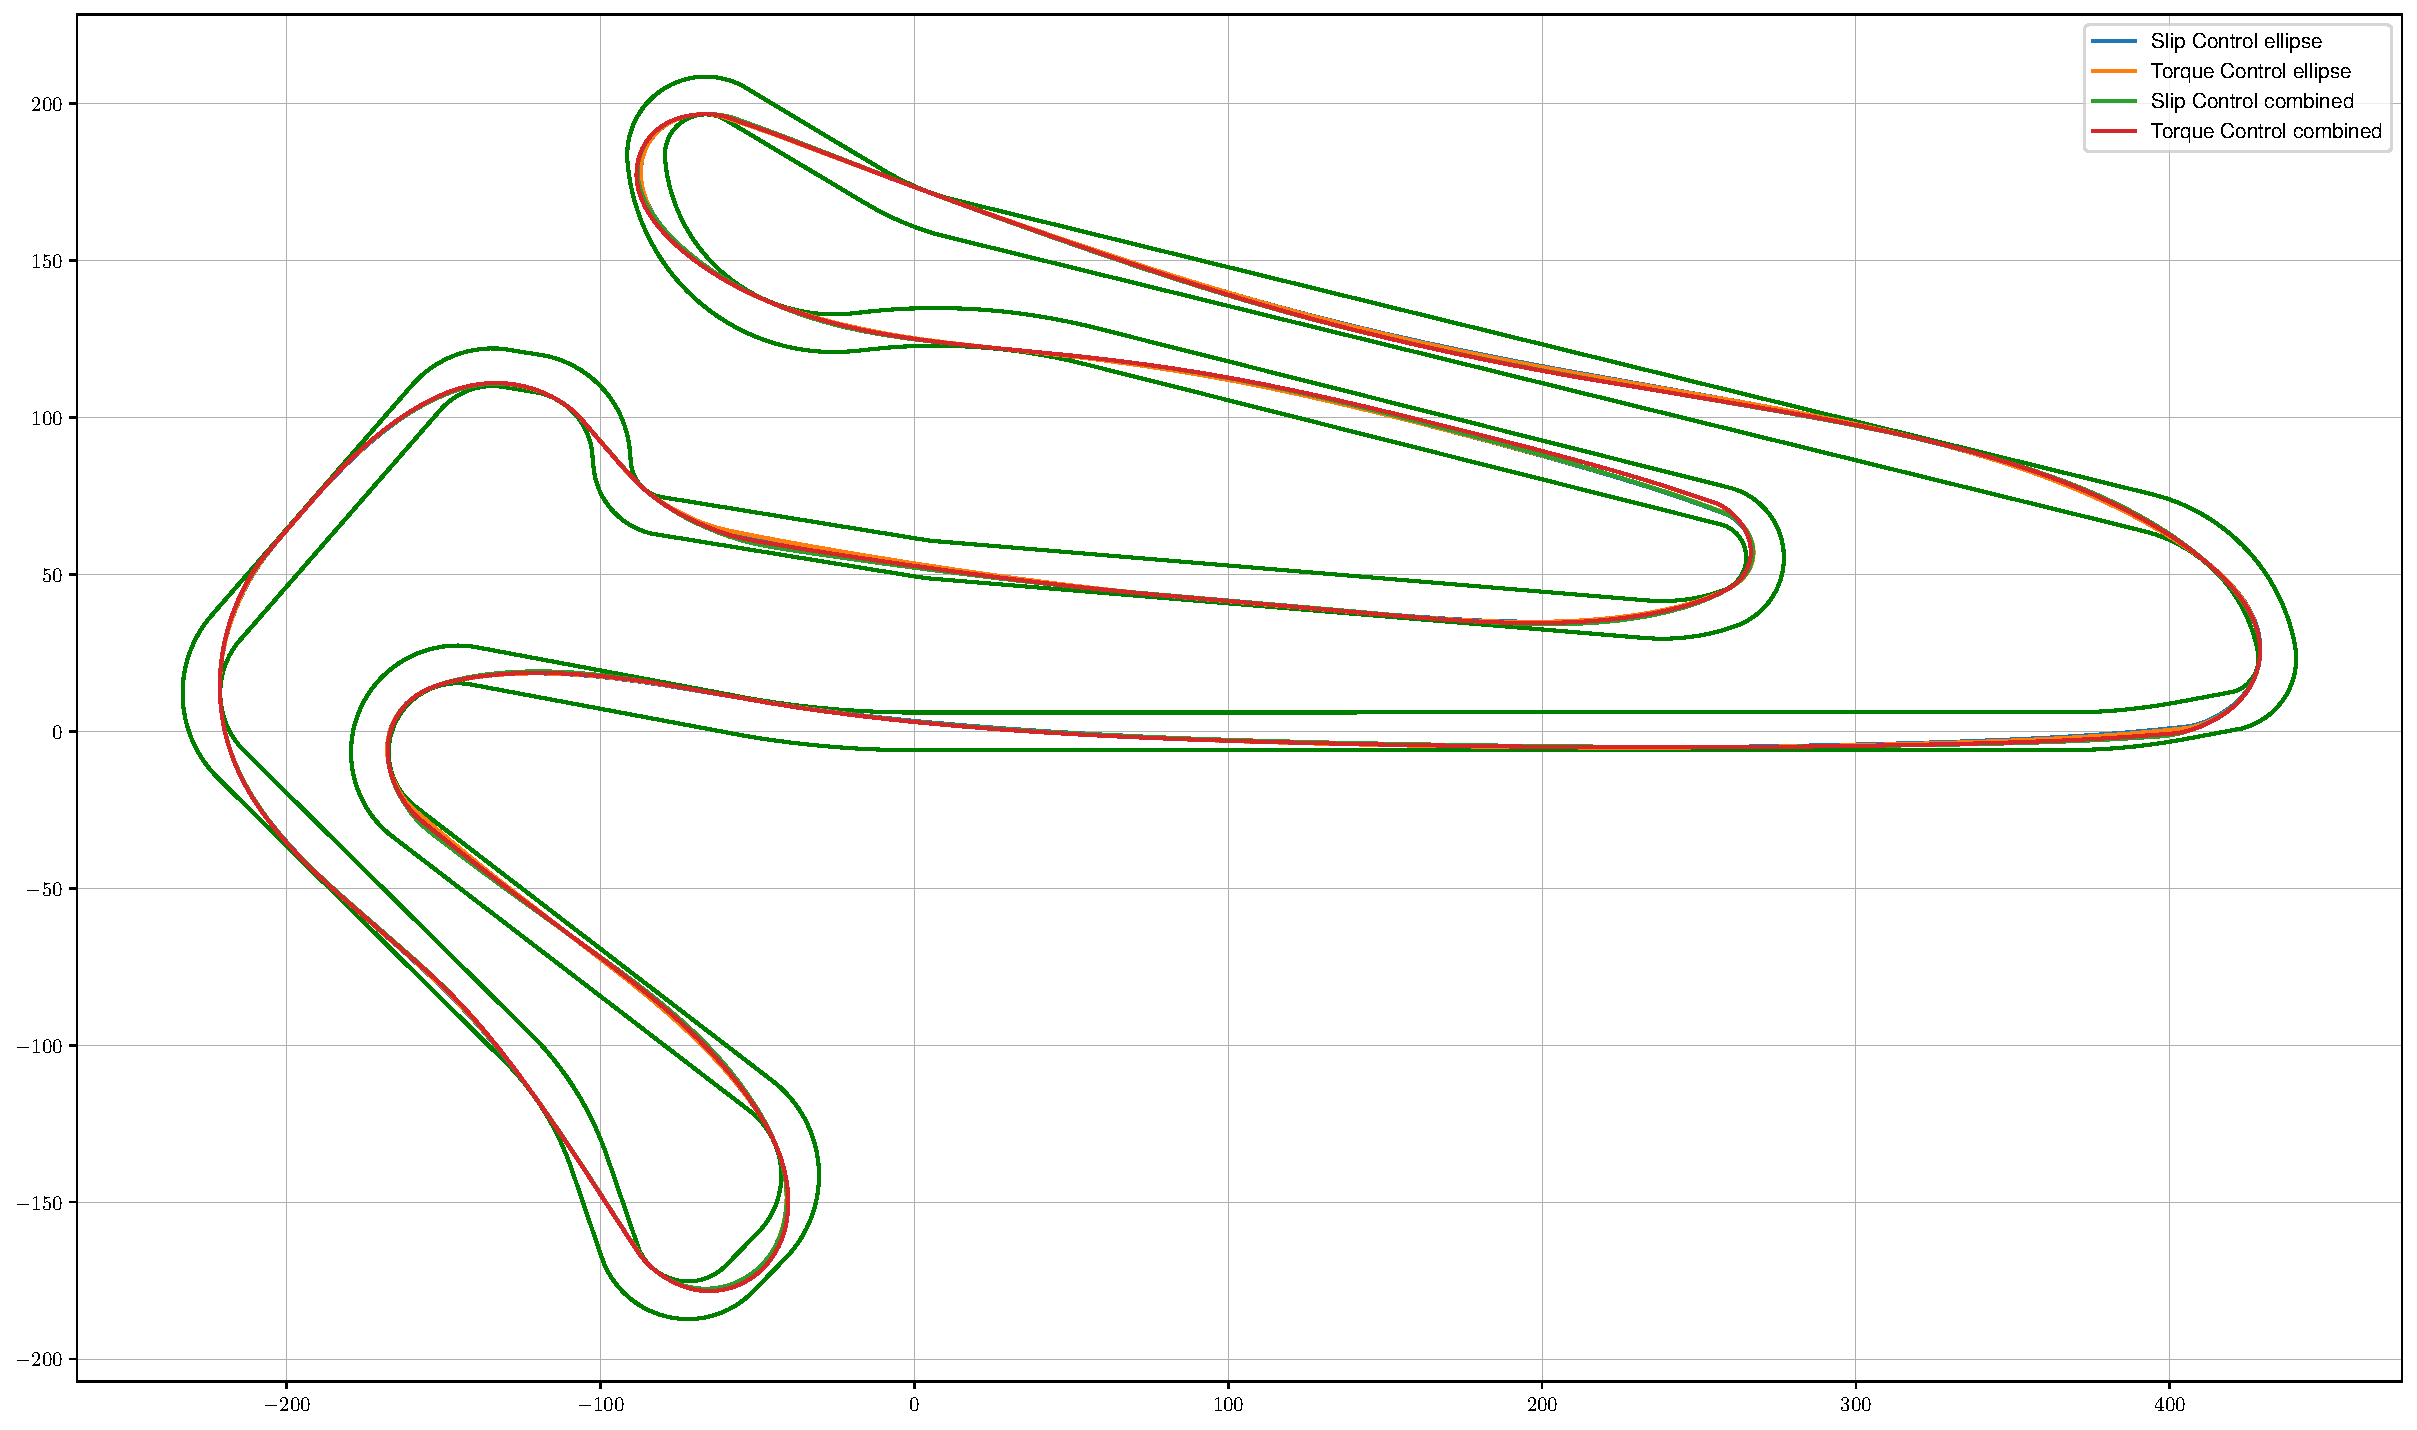
\includegraphics[angle=90,origin=c,height=1\linewidth]{Circuit/Track_P_confront.pdf}
    \caption{Trajectory}
    \label{fig:AdriaTrajConfront}
\end{figure}
%
\clearpage
%